\documentclass[journal,12pt,twocolumn]{IEEEtran}

\title{ASSIGNMENT 1}
\author{Tushita Sharva, CS21BTECH11022}

\usepackage{graphicx}
\usepackage{amsmath}
\usepackage{amssymb}
\begin{document}


\providecommand{\brak}[1]{\ensuremath{\left(#1\right)}}
\newcommand{\question}{\noindent \textbf{Question: }}
\newcommand{\solution}{\noindent \textbf{Solution: }}



\maketitle

\question
Find the value(s) of k for which the quadratic equation $x^2 + 4k x + k^2 - k + 2 = 0$ has equal roots.
\bigskip

\solution
A quadratic equation 
		$$ax^2+bx + c = 0$$

		has equal roots only if 
 the discriminant
		
			$$b^2 - 4a c  = 0$$
			
		Substituting $a = 1,\ b = 4k,\ c = k^2 -k + 2$,
		\begin{align}
		  \brak{4k} ^2 - 4 \brak{k^2 - k + 2}\brak{1} &= 0
		  \\
		  \implies
		  16k^2 - 4k^2+4k-8 = 0
		  \\
		  \implies
		  12k^2 + 4k - 8 = 0
		  \\
		  \implies
		  3k^2 + k - 2 = 0
		\end{align}
		
		On factorising, we get
		\begin{align}
		3k^2 + 3k - 2k - 2 = 0\\
		\implies 3k\brak{k+1}-2\brak{k+1} = 0\\
		\implies \brak{k+1} \brak{3k-2} = 0\\
		\implies k = -1 \ or \ k = \displaystyle\frac{2}{3}
		 \end{align}
		 
		 Check: if $k = -1$
		 \begin{align}
		     x^2 + 4k x + k^2 - k + 2 = 0\\
		     \implies x^2 - 4x + 4 = 0\\
		     \implies \brak{x-2}^2= 0\\
		     \implies x = 2 ,\ 2
		 \end{align}
		 
		 Check: if $k = \displaystyle\frac{2}{3}$
		 \begin{align}
		     x^2 + 4k x + k^2 - k + 2 = 0\\
		     \implies x^2 + \frac{8}{3} + \frac{16}{9} = 0\\
		     \implies \brak{x-\frac{-4}{3}}^2= 0\\
		     \implies x = \displaystyle\frac{-4}{3} ,\ \displaystyle\frac{-4}{3}
		 \end{align}
		 
		 \newpage
		 
		 VERIFICATION USING GRAPHS:
		 
		 \begin{figure}[h!]
		  \centering
		  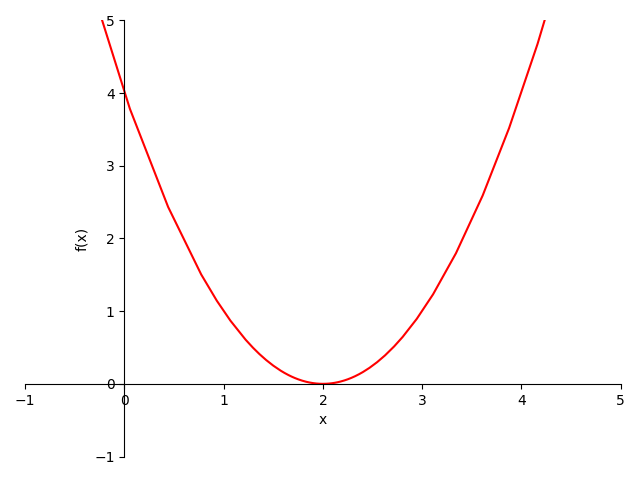
\includegraphics[width = \columnwidth]{Figure_1.png}
		      \caption{Touches the x axis at (2, 0), has equal root "2"}
		      \label{Figure_1}
		 \end{figure}
		 
		 
		\begin{figure}[h!]
		  \centering
		  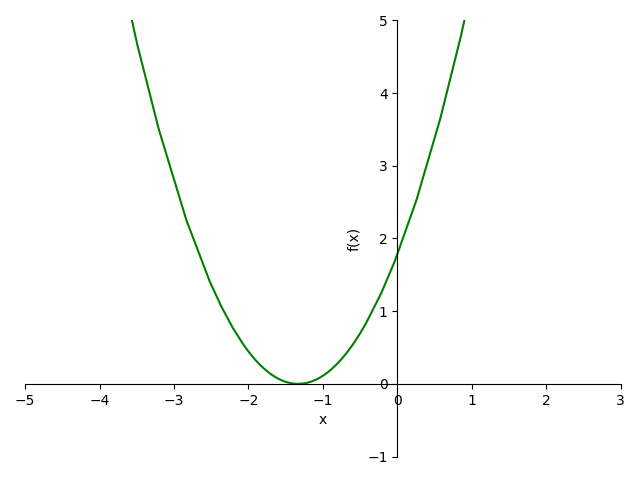
\includegraphics[width = \columnwidth]{Figure_2.png}
		      \caption{Touches the x axis at ($\frac{-4}{3}$, 0), has equal root, $\frac{-4}{3}$}
		      \label{Figure_2}
		 \end{figure}

\end{document}

